% ---------------------------------------------
%                 _   _               _
%  _ __ ___   ___| |_| |__   ___   __| |
% | '_ ` _ \ / _ \ __| '_ \ / _ \ / _` |
% | | | | | |  __/ |_| | | | (_) | (_| |
% |_| |_| |_|\___|\__|_| |_|\___/ \__,_|
% ---------------------------------------------
%* [ ] Fix up xrt.space
%* [ ] Draft design patterns
% ---------------------------------------------
\chapter{A DIY Approach to AR in the Arts}
\label{sec: method}
\markboth{}{A DIY Approach to AR in the Arts}
\epigraph{\emph{This chapter draws some of its content from a published short-paper in the Doctoral Consortium of the Tangible, Embedded, and Embodied Interaction Conference 2021}}{\cite[]{bilbow2021b}}
% ---------------------------------------------
\section{Research Methods}\label{sec: method-methods} % lr > theory > YOU ARE HERE > studies > discussion > conclusion
The methods present in this thesis have stayed consistent with their original proposal, with the exception of specific methods of data collection and analysis being disrupted by the COVID-19 pandemic, which commenced three months after the start of research. 
In \autoref{sec: literature}, the historical origins, contextual trends, exceptions, and contemporary forms of AR technologies were outlined. Additionally, examples of AR's use in the arts were provided, along with specific rationales for their use, e.g. sensory engagement, collaborative expression, and activism and agency. In the previous chapter, I outlined a trio of lenses through which to consider the material, embodied, and spatial aspects of AR. These drew from a 4EC approach to experience, which posits that cognitive processes are embodied, embedded, enacted and extended. In the current chapter I will be outlining my methodological approach to the practice-based side of the research: designing, performing, and evaluating musical AR experiences, and AR DMIs. A review of the outstanding research questions will be outlined, to provide the chapter a clear direction into the ensuing three study chapters.

\begin{enumerate}
    \RQmedium
    \RQexperience
    \RQfuture
\end{enumerate}

The present thesis approaches the above questions by making use of several established practice research methods. Broadly, these methods have lead to practical contributions that will be explored in this chapter and the following three study chapters: namely the creation and iterative design of multisensory AR experiences, and a set of open design patterns for doing so. These practical contributions function both as ongoing research probes, and as platforms for reproducible artistic work for the wider experimental music research community. 

As will be explained in \autoref{sec: method-patterns}, it is within this context of creating, developing, implementing and iterating on a set of open design patterns for AR art and music that the research methods employed in the following chapters are carried out. This started with a motivation for creating smaller (in complexity and in interactable space) experiences, that were simple in their sensory modulation and instrumental reactivity, with the view to later incorporate them in larger scale interactive AR experiences once sufficiently tested. However, due to COVID-19 the prospect of user-testing and iterating on the design of multiple experiences, especially large scale ones, through participant feedback became increasingly difficult to facilitate and plan for. Thus, I opted instead to focus on developing working musical AR prototypes that I myself would play regularly, tweak, and iterate upon. Then, and there, an AR research and compositional practice began.

It's pertinent to mention that practical work, where carried out, has always been documented for analysis, open-research, and archival purposes. I found the combination of \href{https://sambilbow.github.io}{my personal website} as well as \href{https://github.com/sambilbow}{GitHub} a suitable solution for this. Links to project files will be included in the study chapters. Before outlining the aforementioned design patterns, I would first like to touch upon the concept of resistance, and its role in motivating the methodological approach taken in the thesis.



% ---------------------------------------------
\section{Resistance in Practice} \label{sec: method-resistance}
Formative in the development of the methodological approach of this thesis has been the concept of `resistance'. In short, this could be characterised as a motivation for changing or acting against the state of the art, practice, technology, or philosophy, out of a discontent for its status quo. This isn't to be confused by resistance in the sense of experiencing resistance to \textit{do} something, although as might be expected, that has reared its head a few times over the last three years too. Its difficult to place resistance into the linear narrative of this thesis, some resistance formed my initial motivations for the carrying out of this research, and some was garnered along the way, especially around the time of the uptake in `Metaverse' as a term to describe the sum total of all creative XR development. Either way, resistance has made up a large portion of my perspective on AR technologies, its role within digital music and humanities more broadly, and my rationale for pursuing several key areas discussed in the thesis so far (anti-consumerism, multisensory experience, agency), and to come.

As referred to in \autoref{sec: theory-aestheticexperience}, contemporary design research in the fields of computational art and music have in recent years rallied behind the broader ``free/libre and open-source software" and ``open-source hardware" ethoses (abbreviated to FLOSS and OSH respectively). This approach, often hand-in-hand with the Maker, DIY, and Hardware Hacking subcultures, stands in stark contrast to the goings-on of mega-corporations board rooms, with their design `sprints', `agile' workflows, and `human-centred' design. While commentary on the considerable role of un(der)funded volunteer labour involved in OS tools and projects is outside of the scope of this thesis, it is worth mentioning. The approaches taken by these subcultures towards embodied design and composition workflows however, has been highly beneficial for the field. In the case of digital music making, software tools and coding languages like PureData, Maximilian, Supercollider, ixilang, Sonic Pi, TidalCycles, and Bela have granted students, researchers, and composers across disciplines, free and beginner-friendly access to a wealth of tutorials, examples, and tools for advanced real-time sampling and synthesis techniques.

It could be proposed, that this approach is motivated in part by a resistance against many of the `features' typically found in commercial ``closed-source" software and hardware. Providing significant barriers to accessible learning, creativity, and artistic authenticity, these include lack of interoperability with other software, use of proprietary file formats, high initial or recurring subscription costs, and restricted access to lower-level parameters, functions, and settings. It is within this resistance against the closed-source and / or commercial that the practical work of this thesis attempts to situate itself, drawing on its implicit designerly practices and aesthetics. As a result, the path taken to address the key areas of the thesis has involved the bringing into the fore, knowledge from the creative practice of hacking, making, designing, and iterating with experimental and DIY hardware and software.

A second form of resistance that the methodological approach of this thesis explored is the ocularcentrism found in AR technologies mentioned previously in \autoref{sec: literature-interface-sensory-visual} and \autoref{sec: theory-materiality-mediumspec}. As a practitioner of music, and audio related technologies, this has provided a significant portion of the motivation for carrying out the present research, as well as a significant portion of the challenges faced when attempting to develop AR as a medium for sound-based interactive experiences.

Although m

%% wanting to make room for later ms endeavours, time/expertise/cost/access barrier for the moment

%% additive art is inherently hybrid, the space counts etc
%% consumer



% ---------------------------------------------
\section{Design Patterns for AR Art and Music} \label{sec: method-patterns} % The XRt Space acknowledge own resistance and how it leads to bias? guidelines for accessibility etc

The term design pattern here, is borrowed from the field of computer science, where it is taken to describe ``communicating objects and classes that are customized to solve a general design problem in a particular context'' \citep{gamma1995}. A design pattern thus ``names, abstracts, and identifies the key aspects of a common design structure that make it useful for creating a reusable object-oriented design''. So, while as a method it may not operate completely as it would in its native computer science, to address the outstanding aims of the thesis, design patterns do serve to be less rigid than frameworks, more problem-focused than guidelines; whilst inheriting the meaningful organisational structure that comes with an object-oriented design approach\footnote{explain OOD}. Design patterns are characterised by having four elements:
\begin{itemize}
    %*[ ] first two look similar
    \item The \textbf{pattern name} describes the design problem at a higher level of abstraction
    \item The \textbf{problem} describes the situation in which you might apply the pattern
    \item The \textbf{solution} describes the relationships between elements of the pattern that aim to solve the problem
    \item The \textbf{consequences} are the results and trade-offs of applying the pattern
\end{itemize}

\begin{figure}
    \centering
    {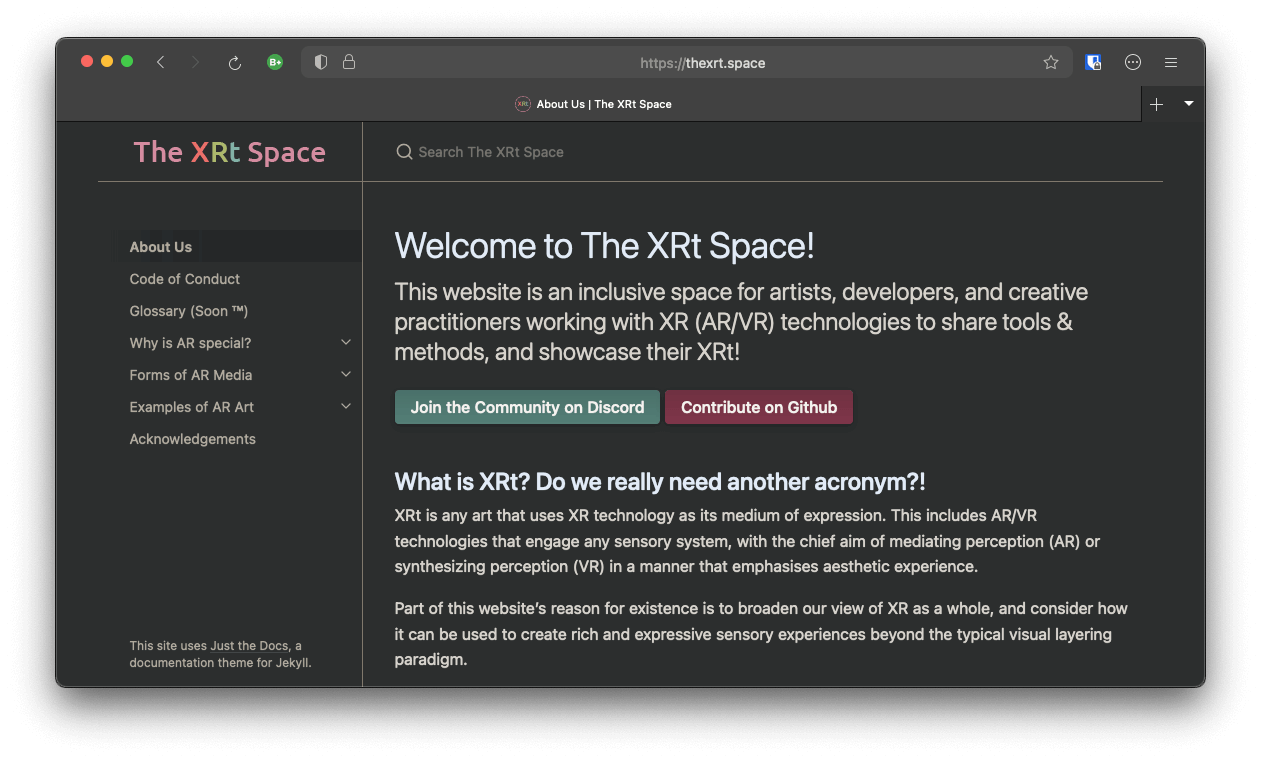
\includegraphics[width=.75\linewidth]{04-method/xrtspace.png}}
    \caption[The XRt Space website]{The XRt Space website}
\end{figure}\label{fig: thexrtspace}

%* [ ] maybe change xrt.space to github.io link
These design patterns are therefore subject to iteration, and the latest version can be found on \href{https://www.thexrt.space}{the XRt Space website}, a community-editable repository created to host and update them. The principles used to guide the patterns draw on the resistances outlined in \autoref{sec: method-resistance}, namely taking a DIY approach, decoupling from the ocularcentric and layering paradigms of typical AR experience, and attempting to navigate an inherently consumerist space whilst trying not to contribute to exploitative systems of oppression that uphold it. They are also guided by the theoretical proposals of \autoref{sec: theory}: that participant's and performer's cognitive processes in the experience of AR artworks are embodied, embedded, enacted, and extended, and have the potential to be modulated to extents that offer novel aesthetic experiences of augmented \hyperref[sec: theory-materiality]{materiality}, \hyperref[sec: theory-embodiment]{embodiment}, and \hyperref[sec: theory-space]{space}. The following sections outline three design patterns, \textit{\nameref*{sec: method-patterns-experience}}, \textit{\nameref*{sec: method-patterns-instrument}}, and \textit{\nameref*{sec: method-patterns-environment}}.

\subsection{Designing for Rich AR Experience} \label{sec: method-patterns-experience} 
\autoref{sec: theory} drew on a number of theoretical propositions, and put forward that AR has the potential to scaffold new modes of performance and expression in the arts and music, furthermore, that from an enactivist approach experience, this would consist in radically modulating the material, embodied, and spatial experience of participants. This is the starting point for ideating and designing an artistic AR experience in the present thesis. This pattern addresses the issue of the typicality of AR experience being simple interactions with visual overlay devices. It approaches experience ideation from a holistic and multisensory, or ``modalities-encompassing'' \citep{schraffenberger2018} perspective. Furthermore, the `4Es' of an enactivist approach can be considered as conditions for what could be described as immersive and ``rich experience" \citep{bilbow2021}. As highlighted in \autoref{sec: theory-materiality-complexitymusic}, enactivist principles have been offered as guidelines for the creation of interactive systems in the past; Essl and O'Modhrain \citeyearpar{essl2006}, Armstrong \citeyearpar{armstrong2006}, and Hayes \citeyearpar{hayes2019} suggest this approach in the design of new musical instruments. 

The concept of rich experience also stands in stark contrast to the current direction of corporate XR technologies, where it is being developed to \textbf{replace} in-person interactions e.g. by facilitating in-headset `work from home' virtual environments such as Meta Horizons. It also stands in contrast with the marketed push towards AR as a tool for driving commerce through targeted advertisements. How as artists and musicians can we avoid the corporate, commercial, ocularcentric, and overlay approach to AR?

\subsubsection{Centre the experience on two or more sensory interactions}
Whether it is Dewey's concept of the ``live creature'', or the contemporary enactivist's framing of the importance of embodiment, the AR experience ought to be \textit{centred on two or more sensory interactions}. It may include any combination of sensory interaction types, i.e visual (vision), auditory (hearing), vestibular (movement and balance), olfactory (smell), gustatory (taste), and somatosensory (touch). %*! add

\subsubsection{Invoke a meaningful relationship between the real and virtual}
AR's medium specificity, discussed in \autoref{sec: theory-materiality-mediumspec}, should be at the forefront of intentional design choices. If AR is unique because its ``invocation of relationships between real and virtual processes in the axes of spatial, thematic, material and ecological distance'', these relationships become a key handle by which artists and musicians can \textit{meaningfully steer experience to achieve aesthetic experiences}. Consider the following:
\begin{itemize}
    \item Spatial \\
    \item Thematic \\
    \item Material \\
    \item Ecological \\
\end{itemize}

\subsubsection{Implement an AR subform from an enactivist perspective}

\subsubsection{Delineate clear spatial and conceptual boundaries for the participant}
Snippets describe a small-scale clip-like \footnote{Similar in scale to the video-clip, sound-clip, clipart, and now app-clip, however conceptually different in that Snippets are not a miniaturised `extracts' or `segments' of a larger experience} AR Experiences that occur in the approximate interaction space of 30cm3, e.g. between a users hands. The Snippet itself does not supply a full sensorial experience, instead providing two human- to-sense interactions through its AR subforms. Rather than being a fully interactive relationship between real and virtual objects / environments (Behavioural Relationship), Snippets contain simpler, and more reactive Content-based Relationships or Spatial Relationships.

Scenes describe medium-scale AR Experiences that occur on and around the body, an approximate interaction space of 200cm3. They can be formed from existing Snippets, or created from scratch. They ideally feature more (and higher complexity) human-to-sense interactions, and therefore potentially more interactive, Content-based and Spatial Relationships between real and virtual elements will be formed.

Spaces describe large-scale AR Experiences, involving multiple human actors in a variety of differently sized interaction spaces in a room. For example, augmented hand / body interaction with the environment and other users, and multiple of zones of interaction in different sections of the room. Spaces provide fully multisensory immersive experiences, by making use of a combination of different sensory modalities, AR subforms, and Behavioural Relationships.


% %[ ] >==> Replace with LaTeX table <==<
% %[ ] >==> Handles / 4EC
% \begin{figure}
%     \centering
%     {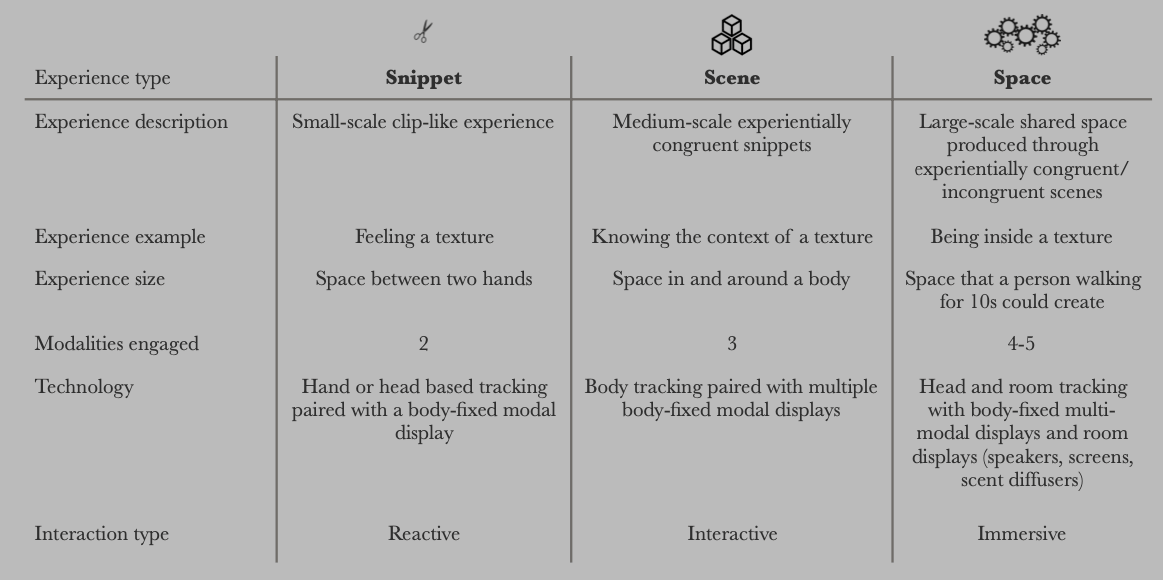
\includegraphics[width=.75\linewidth]{04-method/snippetscenespace.png}}
%     \caption[A Categorisation of AR Interaction Types]{A Categorisation of AR Interaction Types}
% \end{figure}\label{fig: ARinteraction}

\subsection{Consideration of the AR Instrument} \label{sec: method-patterns-instrument}
%[ ]    probably explain the whole experience/piece participant/performer in intro
When describing the means through which a participant or performer meaningfully interacts or engages in any kind of information transfer in the AR system, it is through the AR Instrument. 
%*[ ] >==> Replace with LaTeX table <==<
\begin{figure}
    \centering
    {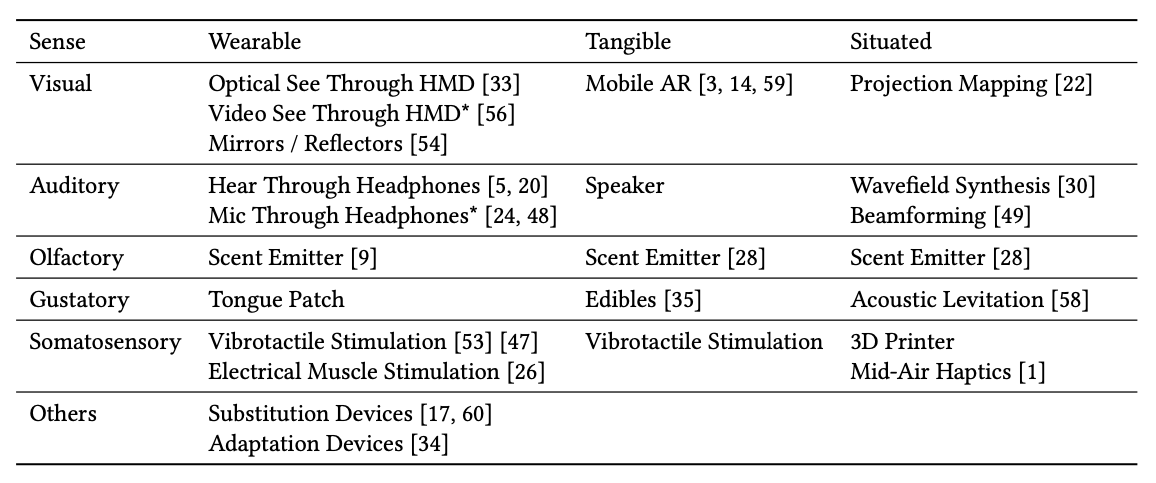
\includegraphics[width=.75\linewidth]{04-method/sensorydisplays.png}}
    \caption[Potential AR Instruments]{Potential AR Instruments}
\end{figure}\label{fig: ARinstrument}
% \begin{table*}
    %     \caption{A classification of potential sensory displays for MSAR Instruments}
    %     \begin{tabular}{lllll}
        %         Sense&Wearable&Tangible&Situated&\\
%         Visual&Optical See Through HMD \tablefootnote{ hi hi\cite{leapmotion2018}}&Mobile AR \tablefootnote{\cite{apple2020,google2020,vuforia2020}}&Projection Mapping \tablefootnote{\cite{lightform2020}} &\\ &Video See Through HMD* \tablefootnote{\cite{varjo2019}}&&&\\ &Mirrors / Reflectors \tablefootnote{\cite{tonn2020}}&&&\\
%         Auditory&Hear Through Headphones \tablefootnote{\cite{kiefer2018,barde2020}}&Speaker&Wavefield Synthesis \tablefootnote{\cite{melchior2005}}&\\&Mic Through Headphones* \tablefootnote{\cite{lindeman2008,sennheiser2018}}&&Beamforming \tablefootnote{\cite{sharma2015}}&\\
%         Olfactory&Scent Emitter \tablefootnote{\cite{brooks2020}}&Scent Emitter \tablefootnote{\cite{maggioni2019}}&Scent Emitter \tablefootnote{\cite{maggioni2019}}&\\
%         Gustatory&Tongue Patch&Edibles \tablefootnote{\cite{narumi2011}}&Acoustic Levitation \tablefootnote{\cite{vi2017}}&\\
%         Somatosensory   &Vibrotactile Stimulation \tablefootnote{\cite{subpac2020}} \tablefootnote{\cite{seah2015}}    &Vibrotactile Stimulation&3D Printer&\\&Electrical Muscle Stimulation \tablefootnote{\cite{lopes2018}}&&Mid-Air Haptics \tablefootnote{\cite{ablart2019}} &\\
%         Others&Substitution Devices \tablefootnote{\cite{ward2010,hafidh2013}}&&&\\ &Adaptation Devices \tablefootnote{\cite{nagel2005}}&&&\\
%     \end{tabular}
% \end{table*}
\subsubsection{Wearable}
Wearable AR Instruments include forms that are worn on the body, including output via head-mounted visual, audio, olfactory and gustatory feedback devices or `displays', and body-mounted proprioceptive feedback devices

\subsubsection{Tangible}
Tangible AR Instruments include forms that can explored by holding or touching, such as devices that use conductive fabrics and textiles to track input, and then providing sensory feedback, e.g. vibrotactile stimulation (somatosensory). They can also be any object that can be granted instrumentality by a device that can track it and provide contextually aware (i.e. corresponding) sensory feedback via another device. For example, a wooden cube could be transformed into a Tangible Instrument through real-time image recognition, and specific interactions with it could provide auditory feedback. In this example, the auditory feedback would likely be delivered via a Wearable Instrument that was also processing the real-time image recognition such as an HMD with bone-conduction headphones.

\subsubsection{Situated}
Situated AR Instruments include forms that are anchored in a real world environment and therefore provide location-specific experiences. Activation is gauged by user enaction, or user presence via infrared camera tracking or proximity of a worn device. Examples of Situated AR Instruments could include an interactive projection mapping with wavefield synthesis providing auditory feedback, and anchored scent emitters providing olfactory feedback

\subsection{Striking a Real-Virtual Balance} \label{sec: method-patterns-environment}
\subsubsection{Choice of Environment}
\subsubsection{Allowance for the Real}
\subsubsection{Believability}



% ---------------------------------------------
\section{AR Experience Studies}
The three ensuing chapters \textit{\nameref{sec: area}}, \textit{\nameref{sec: polaris}}, and \textit{\nameref{sec: polygons}} outline and analyse three different expressive AR DMIs developed over the course of this research, each with different focuses. Though they were initially guided by a loose set of proto-design patterns \citep{bilbow2021b}, it is through the insights and analysis gained through the creation and iteration of their study that the above \hyperref[sec: method-patterns]{design patterns} were developed.

\subsection{Composing area\textasciitilde{} - \autoref{sec: area}}
The starting point for this was the creation of area\textasciitilde{}, a non-visual audio AR experience centred around the self-composition of a hybrid listening environment using an ambisonic microphone, head-, and hand-tracking. As will be expanded upon in \autoref{sec: area}, due to the circumstances of the COVID-19 lockdown, I opted for an autobiographical design method for the iteration and evaluation of the system. Out of the evaluation of this project, namely the endeavour to expand into audiovisual AR experiences, I discovered a suitable platform the develop the rest of doctoral research on: the open-source Project North Star AR headset.

\subsection{Evaluating polaris\textasciitilde{} - \autoref{sec: polaris}}


\subsection{Performing polygons\textasciitilde{} - \autoref{sec: polygons}}
